% makebox for over-wide figure   
\makebox[\linewidth]{
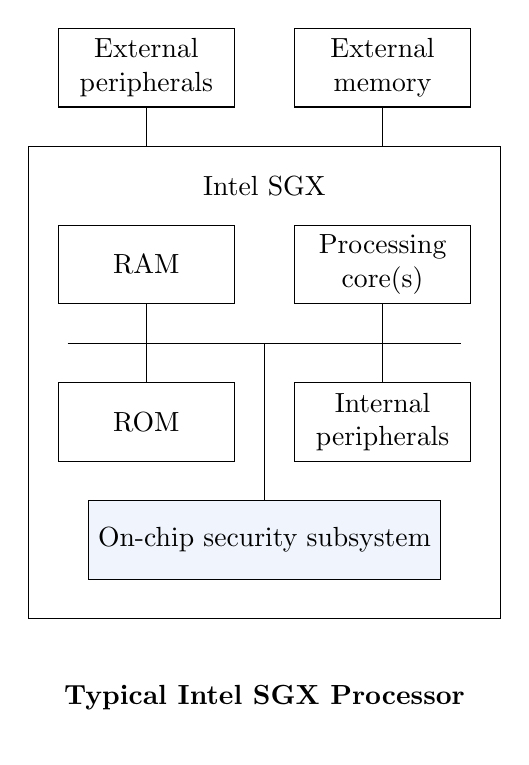
\begin{tikzpicture}[
  transform shape,
  nodes={text width=2cm, draw, minimum height=1cm, align=center},
  tee/.style={fill=CornflowerBlue!10!white},
  subtitle/.style={font=\bfseries, draw=none, text width=}
]
	\node (v1b) at (4.5,1.5) {RAM};
	\node (v2b) at (4.5,-0.5) {ROM};
	\node (v4b) at (7.5,-0.5) {Internal peripherals};
	\node (v3b) at (7.5,1.5) {Processing core(s)};
	\draw (3,3) rectangle (9,-3);
	\node[draw=none] at (6,2.5) {Intel SGX};
	\node (v5b) at (7.5,4) {External memory};
	\node (v7b) at (4.5,4) {External peripherals};
	\node[text width=, tee] (v6b) at (6,-2) {On-chip security subsystem};
	\draw  (3.5,0.5) -- (8.5,0.5);
	\draw  (v1b) |- (4.5,0.5);
	\draw  (v2b) |- (4.5,0.5);
	\draw  (v3b) |- (7.5,0.5);
	\draw  (v4b) |- (7.5,0.5);
	\draw  (v5b) |- (7.5,3);
	\draw  (v7b) |- (4.5,3);
	\draw  (v6b) |- (6,0.5);
	\node[subtitle] at (6,-4) {Typical Intel SGX Processor};
\end{tikzpicture}
}